\documentclass[tikz,border=2pt,11pt]{standalone}
\usetikzlibrary{arrows.meta}
\usetikzlibrary{calc}
\usetikzlibrary{positioning}
\usepackage{amsmath}
\usepackage{amssymb}
\usepackage{tikz}
\usepackage{xcolor}
\newcommand{\kk}{k}
\DeclareMathOperator{\Hom}{Hom}
\DeclareMathOperator{\Ext}{Ext}
\DeclareMathOperator{\End}{End}
\DeclareMathOperator{\rad}{rad}
\DeclareMathOperator{\soc}{soc}
\DeclareMathOperator{\coker}{coker}
\DeclareMathOperator{\im}{im}
\DeclareMathOperator{\id}{id}
\DeclareMathOperator{\Tor}{Tor}
\DeclareMathOperator{\Tr}{Tr}
\newcommand{\stHom}[3]{\underline{\Hom}_{#1}(#2,#3)}
\newcommand{\stEnd}[2]{\underline{\End}_{#1}(#2)}
\newcommand{\D}{\operatorname{D}}
\newcommand{\op}{\mathrm{op}}
\newcommand{\cone}{\operatorname{cone}}
\begin{document}
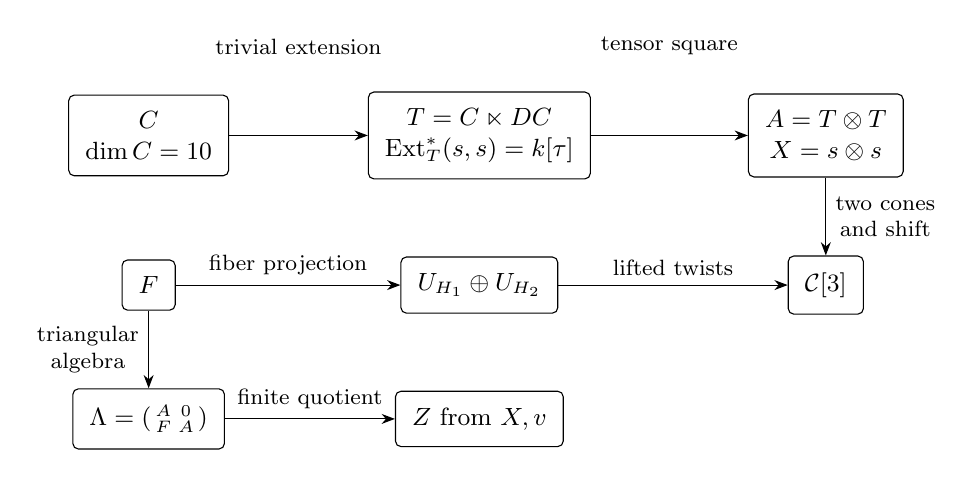
\begin{tikzpicture}[>=Stealth,every node/.style={font=\small},
 box/.style={draw,rounded corners=2pt,inner sep=6pt,align=center},
 lab/.style={font=\footnotesize,align=center}]
\node[box] (c) at (0,3.3) {$C$\\$\dim C=10$};
\node[box] (t) at (4.2,3.3) {$T=C\ltimes DC$\\$\Ext_T^*(s,s)=\kk[\tau]$};
\node[box] (a) at (8.6,3.3) {$A=T\otimes T$\\$X=s\otimes s$};
\node[box] (f) at (0,1.4) {$F$};
\node[box] (u) at (4.2,1.4) {$U_{H_1}\oplus U_{H_2}$};
\node[box] (cone) at (8.6,1.4) {$\mathcal C[3]$};
\node[box] (lam) at (0,-.3) {$\Lambda=\left(\begin{smallmatrix}A&0\\F&A\end{smallmatrix}\right)$};
\node[box] (z) at (4.2,-.3) {$Z$ from $X,v$};
\draw[->] (c)--node[above=9mm,lab]{trivial extension}(t);
\draw[->] (t)--node[above=9mm,lab]{tensor square}(a);
\draw[->] (a)--node[right,lab]{two cones\\and shift}(cone);
\draw[->] (f)--node[above,lab]{fiber projection}(u);
\draw[->] (u)--node[above,lab]{lifted twists}(cone);
\draw[->] (f)--node[left,lab]{triangular\\algebra}(lam);
\draw[->] (lam)--node[above,lab]{finite quotient}(z);
\end{tikzpicture}
\end{document}
